\documentclass[varwidth=true, border=2pt]{standalone}

\usepackage{pgfplots}
\usepackage{tikz}

\usetikzlibrary{calc,patterns,angles,quotes}

\begin{document}
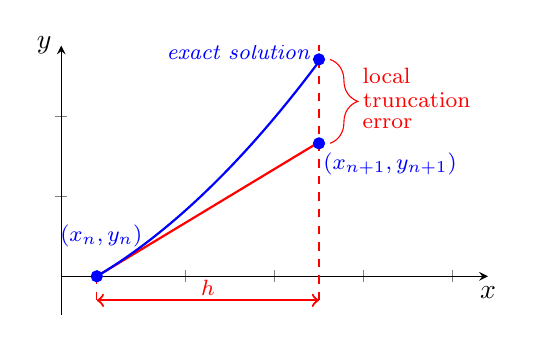
\begin{tikzpicture}
    \begin{axis}[
        legend pos=south east,
        axis x line=middle,
        axis y line=middle,
	every axis x label/.style={at={(current axis.right of origin)},anchor=north},
	every axis y label/.style={at={(current axis.above origin)},anchor=east},
	xticklabels=\empty,
	yticklabels=\empty
        grid = none ,
        width=7cm,
        height=5cm,
        grid style={dashed, gray!1},
        xmin=1,     % start the diagram at this x-coordinate
        xmax=3,    % end   the diagram at this x-coordinate
        ymin=-0.1 ,   % start the diagram at this y-coordinate
        ymax= 1.3,   % end   the diagram at this y-coordinate
        %axis background/.style={fill=white},
        xlabel=$x$,
        ylabel=$y$,
        %xticklabels={-2,-1.6,...,2},
        %yticklabels={-8,-7,...,8},
        %tick align=outside
        enlargelimits=true,
        tension=0.08]


          \addplot[domain=1:2.25, red, thick,samples=250] {0.67*(x-1)};
        	\addplot[domain=1:2.25, blue, thick,samples=250] {0.33*x^2 -0.33}; % Parabola
        	\addplot[dashed,red,mark=none] coordinates{(2.25,-0.15)(2.25,2)} node[below, pos=0] {}; %x1
	\addplot[dashed,red,mark=none] coordinates{(1,-0.15)(1,0.05)} node[below, pos=0] {}; %x1
  %      \addplot[domain=0.7:1.65, red, thick,samples=250] {1.5*x-1.25}; % Tangent Line


%	\addplot[dashed,red,mark=none] coordinates{(1.25,0)(1.25,0.625)} node[below, pos=0] {$x_0$}; %x0
	\addplot[blue, only marks, mark=*] coordinates {(1,0)(2.25,0.83)(2.25,1.354)};
	\node(L)[red] at (axis cs: 2.63,1.25){\footnotesize{local}};
	\node(T)[red] at (axis cs: 2.8,1.1){\footnotesize{truncation}};
	\node(E)[red] at (axis cs: 2.635,0.95){\footnotesize{error}};
	\node(ES)[blue] at (axis cs: 1.8,1.4){\footnotesize{\textit{exact solution}}};
	\node(x2)[blue] at (axis cs: 2.65,0.7){\footnotesize{$(x_{n+1},y_{n+1})$}};
	\node(x3)[blue] at (axis cs: 1.025,0.25){\footnotesize{$(x_n,y_n)$}};
	\node(h)[red] at (axis cs: 1.625,-0.07){\footnotesize{$h$}};

	\draw [red, decorate,decoration={brace,amplitude=10pt,mirror,raise=4pt},yshift=0pt]
	(axis cs: 2.25,0.83) -- (axis cs: 2.25,1.354) node [red,midway,xshift=0.8cm] {};
	
	\draw [thick,red, <->] (axis cs: 1, -0.15) to (axis cs: 2.25, -0.15);
    \end{axis}
\end{tikzpicture}
\end{document}